\chapter[XÂY DỰNG MÔ HÌNH PHÁT HIỆN TIN TỨC GIẢ MẠO]{Xây dựng mô hình phát hiện tin tức giả mạo}

Chương này trình bày toàn bộ quá trình xây dựng mô hình phát hiện tin tức giả mạo: từ mô tả bộ dữ liệu, quy trình tiền xử lý, vector hóa, thiết kế thí nghiệm, thuật toán KNN trong đề tài, tới kết quả thực nghiệm, đánh giá, phân tích lỗi và ứng dụng demo.

\section{Mô tả bộ dữ liệu}

\subsection{Nguồn gốc bộ dữ liệu}

Đề tài sử dụng bộ dữ liệu \textbf{ISOT Fake News} \cite{ahmed2017}, được nhóm nghiên cứu Information Security and Object Technology (ISOT), Trường Đại học Victoria (Canada) công bố và được chia sẻ rộng rãi trên nền tảng Kaggle \cite{dataset}. Bộ dữ liệu gồm hai tệp tin:

\begin{itemize}
    \item \textbf{Fake.csv}: 23.481 bài tin tức giả, thu thập từ các trang web chuyên đăng tin không xác thực như LosingForReal, Breitbart, NewswithViews,\ldots
    \item \textbf{True.csv}: 21.417 bài tin tức thật, thu thập chủ yếu từ báo chí chính thống như Reuters, The Wall Street Journal, Bloomberg,\ldots
\end{itemize}

Lưu ý: con số trong tệp tải về từ Kaggle (23.481 + 21.417 = 44.898 bài) có thể chênh lệch nhẹ so với mô tả ban đầu của nhóm tác giả \cite{ahmed2017} do bộ dữ liệu được cập nhật theo thời gian.

Mỗi bản ghi gồm các trường thông tin được mô tả trong bảng \ref{tab:mo-ta-du-lieu}.

\begin{table}[H]
\centering
\caption{Mô tả các trường dữ liệu trong bộ dữ liệu ISOT}
\label{tab:mo-ta-du-lieu}
\begin{tabular}{|p{3cm}|p{5cm}|p{4.5cm}|}
\hline
\textbf{Trường dữ liệu} & \textbf{Mô tả} & \textbf{Ví dụ} \\
\hline
title & Tiêu đề bài viết & ``WATCH: Firefighter Catches Baby Dropped From Building'' \\
\hline
text & Nội dung toàn văn bài viết & ``The latest round of bogus testimony\ldots'' \\
\hline
subject & Chủ đề bài viết & politics, world news, government news, left-news, US News, Middle-east \\
\hline
date & Ngày đăng & April 21, 2017 \\
\hline
\end{tabular}
\Nguon{Bộ dữ liệu ISOT Fake News \cite{ahmed2017}}
\end{table}

\subsection{Thống kê mô tả dữ liệu}

Gộp hai tệp được \textbf{44.898 bài viết}. Nhóm tiến hành thống kê một số đặc điểm cơ bản của bộ dữ liệu (bảng \ref{tab:thong-ke-du-lieu}); các chỉ số tính trên bộ dữ liệu sau khi loại bỏ trùng lặp được trình bày ngay dưới bảng.

\begin{table}[H]
\centering
\caption{Thống kê mô tả bộ dữ liệu ISOT}
\label{tab:thong-ke-du-lieu}
\begin{tabular}{|l|c|c|}
\hline
\textbf{Chỉ số} & \textbf{Tin thật} & \textbf{Tin giả} \\
\hline
Số lượng bài viết (tệp gốc) & 21.417 & 23.481 \\
\hline
Sau loại bỏ trùng lặp / rỗng & 21.197 & 17.908 \\
\hline
Tỷ lệ trong bộ dữ liệu sử dụng & 54,2\% & 45,8\% \\
\hline
Số từ trung bình / bài viết & 396 & 438 \\
\hline
Số chủ đề (subject) & 2 & 6 \\
\hline
Khoảng thời gian đăng & 2016--2017 & 2015--2017 \\
\hline
\end{tabular}
\Nguon{Nhóm tự thống kê trên dữ liệu ISOT}
\end{table}

Sau bước kiểm tra trùng lặp và giá trị rỗng, bộ dữ liệu sử dụng gồm \textbf{39.105 bài viết} (loại bỏ 5.573 bài giả và 220 bài thật trùng lặp), hai lớp ở trạng thái gần cân bằng (54,2\%/45,8\%) nên không cần áp dụng các kỹ thuật cân bằng dữ liệu (oversampling, SMOTE\ldots). Bộ dữ liệu được chia ngẫu nhiên theo tỷ lệ \textbf{75\% tập huấn luyện} (29.328 bài) và \textbf{25\% tập kiểm tra} (9.777 bài). Quan sát đáng chú ý: tin giả có độ dài trung bình lớn hơn tin thật (438 so với 396 từ) và đa dạng chủ đề hơn hẳn (6 so với 2 chủ đề) --- đây là những đặc điểm có thể giúp mô hình phân biệt hai lớp.

\begin{figure}[H]
    \centering
    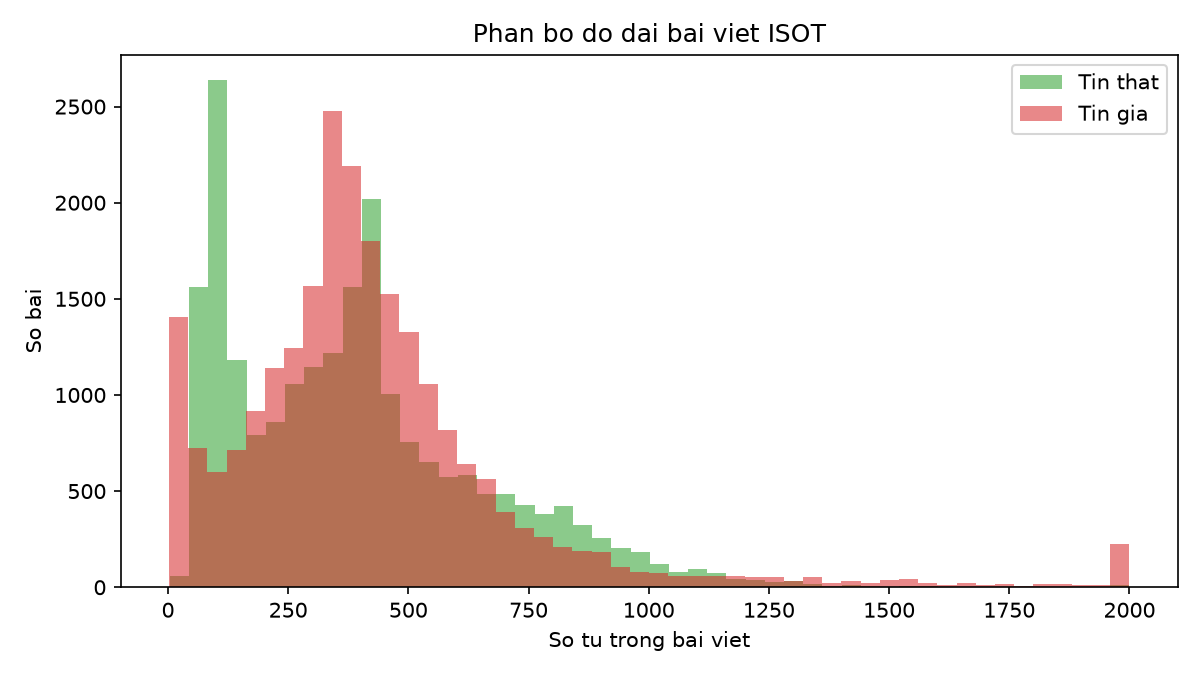
\includegraphics[width=0.85\textwidth]{images/phan-bo-do-dai.png}
    \caption{Phân bố độ dài bài viết của hai lớp tin thật và tin giả}
    \label{fig:phan-bo-do-dai}
    \Nguon{Nhóm tự thực hiện trên dữ liệu ISOT}
\end{figure}

Ngoài ra, nhóm kiểm tra dữ liệu trùng lặp và giá trị thiếu; các bài viết trùng lặp hoặc có nội dung rỗng được loại bỏ trước khi chia tập huấn luyện/kiểm tra để tránh rò rỉ dữ liệu (data leakage) giữa hai tập.

\section{Quy trình xử lý tổng thể}

Quy trình xây dựng mô hình trong đề tài gồm 6 bước, được trình bày tại sơ đồ \ref{sodo:quy-trinh}.

\begin{sodo}[H]
    \centering
    \begin{tikzpicture}[>=stealth, font=\small]
        \node[draw, text width=3.2cm, align=center] (data) at (0,0)
            {Thu thập dữ liệu\\ ISOT Fake News};
        \node[draw, text width=3.2cm, align=center] (pre) at (4.4,0)
            {Tiền xử lý\\ văn bản};
        \node[draw, text width=3.2cm, align=center] (feat) at (8.8,0)
            {Vector hóa\\ TF-IDF};
        \node[draw, text width=3.2cm, align=center] (train) at (8.8,-2.6)
            {Xây dựng\\ mô hình KNN};
        \node[draw, text width=3.2cm, align=center] (eval) at (4.4,-2.6)
            {Đánh giá trên\\ tập kiểm tra};
        \node[draw, text width=3.2cm, align=center] (out) at (0,-2.6)
            {Kết quả:\\ Tin thật / Tin giả};
        \draw[->, thick] (data) -- (pre);
        \draw[->, thick] (pre) -- (feat);
        \draw[->, thick] (feat) -- (train);
        \draw[->, thick] (train) -- (eval);
        \draw[->, thick] (eval) -- (out);
    \end{tikzpicture}
    \SodoCaption{Quy trình xây dựng mô hình phát hiện tin tức giả mạo}{Nhóm tự xây dựng}
    \label{sodo:quy-trinh}
\end{sodo}

\section{Tiền xử lý dữ liệu}

Bộ dữ liệu gốc là văn bản tự do, chứa nhiều yếu tố nhiễu không phục vụ việc phân loại. Các bước tiền xử lý được thực hiện như sau:

\begin{enumerate}
    \item \textbf{Gộp và gán nhãn}: đọc hai tệp Fake.csv và True.csv, gán nhãn $1$ cho tin giả, $0$ cho tin thật; giữ lại hai trường title và text, ghép thành một trường nội dung.
    \item \textbf{Làm sạch văn bản}: chuyển về chữ thường; loại bỏ thẻ HTML, đường dẫn URL, dấu câu, ký tự đặc biệt và chữ số.
    \item \textbf{Tách từ và loại từ dừng}: tách văn bản thành danh sách từ, loại bỏ các từ dừng tiếng Anh (sử dụng bộ từ dừng của thư viện NLTK).
    \item \textbf{Rút gọn từ}: đưa từ về gốc bằng thuật toán Porter Stemmer.
\end{enumerate}

\begin{table}[H]
\centering
\caption{Ví dụ kết quả tiền xử lý một văn bản}
\label{tab:vi-du-tien-xu-ly}
\begin{tabular}{|p{3.2cm}|p{10cm}|}
\hline
\textbf{Bước} & \textbf{Kết quả} \\
\hline
Văn bản gốc & ``As U.S. budget fight looms, Republicans flip their fiscal message\ldots'' \\
\hline
Chữ thường, bỏ ký tự đặc biệt & ``as us budget fight looms republicans flip their fiscal message'' \\
\hline
Loại từ dừng & ``us budget fight looms republicans flip fiscal message'' \\
\hline
Stemming & ``us budget fight loom republican flip fiscal messag'' \\
\hline
\end{tabular}
\Nguon{Nhóm tự thực hiện trên dữ liệu ISOT}
\end{table}

\section{Vector hóa dữ liệu}

Sau tiền xử lý, văn bản cần được chuyển thành dạng số. Nhóm sử dụng \textbf{TF-IDF} (cơ sở lý thuyết tại mục \ref{sec:tfidf} chương 2; tham số hóa qua TfidfVectorizer của thư viện scikit-learn \cite{sklearn}) với cấu hình:

\begin{itemize}
    \item \textbf{n-gram $(1, 2)$}: đặc trưng gồm cả từ đơn (unigram) và cặp từ liên tiếp (bigram), giúp giữ lại một phần ngữ nghĩa kiểu ``breaking news'', ``fake witness''.
    \item \textbf{max\_features $= 50.000$}: chỉ giữ lại 50.000 n-gram có tần suất tài liệu cao nhất, loại bỏ các n-gram quá hiếm chỉ gây nhiễu và tốn bộ nhớ.
    \item \textbf{Chuẩn hóa L2} (mặc định): mỗi vector văn bản được chia cho độ dài Euclidean của chính nó, đưa mọi bài về cùng một thang đo bất kể độ dài --- điều kiện quan trọng để khoảng cách cosine phản ánh đúng độ tương đồng giữa các bài viết.
\end{itemize}

Ma trận đặc trưng cuối cùng có kích thước \textbf{29.328 $\times$ 50.000} (rất thưa: mỗi bài chỉ dùng tới vài trăm n-gram). Vectorizer được \textbf{fit trên tập huấn luyện} rồi chỉ \textit{transform} tập kiểm tra, bảo đảm không có thông tin từ tập kiểm tra rò rỉ vào bước xây dựng đặc trưng. Cùng một ma trận TF-IDF được dùng cho cả bốn mô hình (KNN và ba mô hình tham chiếu), bảo đảm so sánh công bằng giữa các thuật toán.

\section{Thuật toán KNN trong đề tài}

\subsection{Cấu hình mô hình}

Mô hình chính của đề tài là KNN với cấu hình được tổng hợp trong bảng \ref{tab:tham-so-mo-hinh}.

\begin{table}[H]
\centering
\caption{Cấu hình thuật toán KNN}
\label{tab:tham-so-mo-hinh}
\begin{tabular}{|l|l|}
\hline
\textbf{Thành phần} & \textbf{Giá trị lựa chọn} \\
\hline
Đặc trưng đầu vào & TF-IDF (n-gram $1$--$2$, 50.000 đặc trưng) \\
\hline
Số láng giềng $k$ & 5 \\
\hline
Phép đo khoảng cách & Cosine \\
\hline
Trọng số láng giềng & Theo khoảng cách ($w_i = 1/d_i$) \\
\hline
Cách tìm láng giềng & Brute force (quét toàn bộ tập huấn luyện) \\
\hline
Ngưỡng quyết định & 0,5 (theo tỷ lệ trọng số bỏ phiếu) \\
\hline
Tỷ lệ chia dữ liệu & 75\% huấn luyện / 25\% kiểm tra \\
\hline
\end{tabular}
\Nguon{Nhóm tự xây dựng (thư viện scikit-learn \cite{sklearn})}
\end{table}

Các lựa chọn trên được kiểm chứng qua các thí nghiệm ở mục \ref{sec:kq-thuc-nghiem}: $k = 5$ nằm trong vùng cấu hình ổn định của đường cong theo $k$ (E3); cosine là phép đo phù hợp cho vector TF-IDF chuẩn hóa (E4); trọng số theo khoảng cách nhỉnh hơn trọng số đều (E5).

\subsection{Sơ đồ hoạt động khi dự đoán}

Sơ đồ \ref{sodo:kien-truc} mô tả luồng xử lý khi mô hình kiểm tra một bài tin tức mới.

\begin{sodo}[H]
    \centering
    \begin{tikzpicture}[>=stealth, font=\small]
        \node[draw, text width=3.0cm, align=center] (n1) at (0,0)
            {Bài tin mới\\ (tiêu đề + nội dung)};
        \node[draw, text width=3.0cm, align=center] (n2) at (3.85,0)
            {Tiền xử lý\\ (làm sạch văn bản)};
        \node[draw, text width=3.0cm, align=center] (n3) at (7.7,0)
            {Vector TF-IDF\\ (50.000 chiều, chuẩn hóa L2)};
        \node[draw, text width=3.0cm, align=center] (n4) at (11.55,0)
            {Tính khoảng cách cosine\\ tới 29.328 bài huấn luyện};
        \node[draw, text width=3.0cm, align=center] (n5) at (11.55,-2.7)
            {Chọn 5 láng giềng\\ gần nhất};
        \node[draw, text width=3.0cm, align=center] (n6) at (7.7,-2.7)
            {Bỏ phiếu có trọng số\\ ($w_i = 1/d_i$)};
        \node[draw, text width=3.0cm, align=center] (n7) at (3.85,-2.7)
            {Kết quả: nhãn\\ + xác suất tin giả};
        \draw[->, thick] (n1) -- (n2);
        \draw[->, thick] (n2) -- (n3);
        \draw[->, thick] (n3) -- (n4);
        \draw[->, thick] (n4) -- (n5);
        \draw[->, thick] (n5) -- (n6);
        \draw[->, thick] (n6) -- (n7);
    \end{tikzpicture}
    \SodoCaption{Luồng xử lý khi KNN dự đoán một bài tin tức mới}{Nhóm tự xây dựng}
    \label{sodo:kien-truc}
\end{sodo}

Xác suất ``tin giả'' mà hệ thống hiển thị cho người dùng chính là \textbf{tỷ lệ trọng số} của các láng giềng thuộc lớp tin giả trong $k = 5$ láng giềng gần nhất:
\begin{equation}
    \hat{p}(\text{giả}) = \frac{\sum_{i \in N_k(x),\, y_i = 1} 1/d_i}{\sum_{i \in N_k(x)} 1/d_i},
    \label{eq:xac-suat-knn}
\end{equation}
và bài viết được cảnh báo là tin giả khi $\hat{p}(\text{giả}) \geq 0{,}5$. Cơ chế này cho phép ứng dụng hiển thị ``độ tin cậy'' liên tục thay vì chỉ nhãn cứng, đồng thời là đầu vào cho đường cong ROC ở phần đánh giá.

\subsection{Đặc điểm lazy learning của KNN}

Điểm khác biệt căn bản của KNN so với các mô hình tham chiếu nằm ở phân bổ chi phí tính toán. Bước ``huấn luyện'' của KNN chỉ là \textbf{ghi nhớ} ma trận TF-IDF của tập huấn luyện --- gần như tốn 0 giây; ngược lại, mỗi lần dự đoán phải tính khoảng cách từ bài cần kiểm tra tới \textit{tất cả} 29.328 bài huấn luyện (độ phức tạp $O(n_{\text{train}} \cdot d)$ mỗi mẫu). Với 9.777 bài kiểm tra, tổng chi phí dự đoán lên tới hàng phút --- chậm hơn khoảng \textbf{9.000 lần} mô hình tuyến tính, vốn trả trọn ``tiền học'' trong vài phần mươi giây huấn luyện và dự đoán gần như tức thì. Sự đánh đổi này được đo đạc và phân tích cụ thể ở mục \ref{sec:kq-thuc-nghiem} và \ref{sec:nhan-xet}.

\section{Thiết kế thí nghiệm}

\subsection{Mô hình tham chiếu}

Để có cơ sở so sánh, đề tài xây dựng song song ba mô hình học máy truyền thống trên cùng bộ dữ liệu, sử dụng đúng ma trận đặc trưng TF-IDF (n-gram $n = 1..2$):

\begin{itemize}
    \item \textbf{Multinomial Naive Bayes}: mô hình xác suất dựa trên định lý Bayes, giả định các đặc trưng độc lập.
    \item \textbf{Logistic Regression}: mô hình phân loại tuyến tính cho nhị phân, tiêu biểu cho các phương pháp dựa trên đặc trưng TF-IDF.
    \item \textbf{Passive Aggressive}: mô hình học trực tuyến, là mô hình tham chiếu trong nghiên cứu gốc của bộ dữ liệu \cite{ahmed2017}.
\end{itemize}

\subsection{Kịch bản thí nghiệm}

Thí nghiệm được thiết kế gồm các kịch bản:

\begin{table}[H]
\centering
\caption{Các kịch bản thí nghiệm}
\label{tab:kich-ban}
\begin{tabular}{|c|p{5.5cm}|p{5.5cm}|}
\hline
\textbf{STT} & \textbf{Kịch bản} & \textbf{Mục đích} \\
\hline
E1 & Xây dựng 3 mô hình tham chiếu với TF-IDF & Xây dựng baseline so sánh \\
\hline
E2 & KNN cấu hình chuẩn (bảng \ref{tab:tham-so-mo-hinh}) & Mô hình chính của đề tài \\
\hline
E3 & Thay đổi số láng giềng: $k = 1 / 3 / 5 / 7 / 9 / 11$ & Ảnh hưởng của tham số $k$ \\
\hline
E4 & Thay đổi phép đo khoảng cách: cosine / euclidean & Ảnh hưởng của thước đo tương đồng \\
\hline
E5 & Thay đổi trọng số láng giềng: distance / uniform & Ảnh hưởng của cơ chế bỏ phiếu \\
\hline
E6 & Thay đổi cách biểu diễn: BoW / TF-IDF (unigram, 1--2gram, min\_df, số chiều) & Chọn cách vector hóa cho mô hình chính \\
\hline
\end{tabular}
\Nguon{Nhóm tự xây dựng}
\end{table}

Mỗi kịch bản được chạy với cùng một cách chia dữ liệu (cố định random seed) để bảo đảm so sánh công bằng. Đánh giá được thực hiện trên tập kiểm tra chiếm 25\% dữ liệu mà mô hình chưa từng thấy.

\subsection{Công cụ và môi trường thực nghiệm}

\begin{table}[H]
\centering
\caption{Công cụ và môi trường thực nghiệm}
\label{tab:moi-truong}
\begin{tabular}{|l|l|}
\hline
\textbf{Thành phần} & \textbf{Công cụ} \\
\hline
Ngôn ngữ lập trình & Python 3.12 \\
\hline
Thư viện học máy & scikit-learn (KNN, Naive Bayes, Logistic Regression, Passive Aggressive) \\
\hline
Thư viện xử lý ngôn ngữ & NLTK \\
\hline
Thư viện trực quan hóa & Matplotlib, Seaborn \\
\hline
Môi trường thực thi & Máy tính cá nhân (CPU, hệ điều hành Windows) \\
\hline
\end{tabular}
\Nguon{Nhóm tự tổng hợp}
\end{table}

\section{Kết quả thực nghiệm}
\label{sec:kq-thuc-nghiem}

% Số liệu dưới đây là kết quả chạy thực tế của nhóm (log scikit-learn).
\subsection{Kết quả trên tập kiểm tra}

Bảng \ref{tab:ket-qua} tổng hợp kết quả của bốn mô hình trên tập kiểm tra (25\% dữ liệu, 9.777 bài).

\begin{table}[H]
\centering
\caption{Kết quả phân loại của các mô hình trên tập kiểm tra}
\label{tab:ket-qua}
\begin{tabular}{|l|c|c|c|c|}
\hline
\textbf{Mô hình} & \textbf{Accuracy (\%)} & \textbf{Precision (\%)} & \textbf{Recall (\%)} & \textbf{F1 (\%)} \\
\hline
Naive Bayes + TF-IDF & 95,81 & 95,31 & 95,39 & 95,35 \\
\hline
Logistic Regression + TF-IDF & 98,84 & 99,29 & 98,14 & 98,71 \\
\hline
Passive Aggressive + TF-IDF & \textbf{99,37} & \textbf{99,48} & \textbf{99,11} & \textbf{99,30} \\
\hline
\textbf{KNN (mô hình đề xuất)} & 89,35 & 93,24 & 82,34 & 87,45 \\
\hline
\end{tabular}
\Nguon{Nhóm tự thực hiện}
\end{table}

Kết quả cho thấy cả ba mô hình tham chiếu đều vượt xa mức $\sim$93\% của Passive Aggressive trong nghiên cứu gốc \cite{ahmed2017} trên cùng bộ dữ liệu, với \textbf{Passive Aggressive đạt cao nhất (99,37\%)}. Các mô hình tuyến tính TF-IDF đạt gần 99\% là một tín hiệu quan trọng: bộ dữ liệu ISOT thu tin thật và tin giả từ hai nhóm nguồn khác biệt (Reuters so với các trang đăng tin giả), nên nhiều từ --- tên chủ đề, kiểu văn phong, cách viết tiêu đề --- gắn chặt với từng lớp, khiến mô hình học ranh giới toàn cục trên tần suất từ phân loại được gần như hoàn hảo.

KNN đạt \textbf{89,35\%} --- thấp nhất trong bốn mô hình, thấp hơn Passive Aggressive 10 điểm phần trăm. Đây là kết quả đặc trưng của KNN trên dữ liệu văn bản: thay vì học một ranh giới quyết định toàn cục, KNN quyết định theo láng giềng cục bộ, nên dễ bị ảnh hưởng bởi những bài viết có từ vựng giao thoa giữa hai lớp và bởi các mẫu nhiễu (phân tích chi tiết ở mục \ref{sec:nhan-xet} và phần kịch bản thí nghiệm). Dù vậy, 89,35\% là mức không tồi đối với một thuật toán \textit{hoàn toàn không thực hiện học}: toàn bộ hiệu năng đến từ việc so khớp trực tiếp với các bài viết đã biết.

Hình \ref{fig:confusion} là ma trận nhầm lẫn của mô hình KNN trên tập kiểm tra.

\begin{figure}[H]
    \centering
    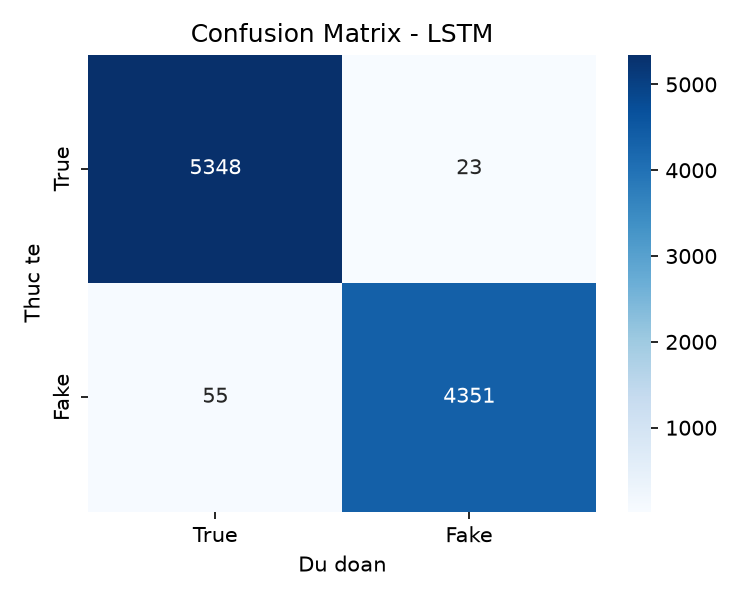
\includegraphics[width=0.75\textwidth]{images/confusion-matrix.png}
    \caption{Ma trận nhầm lẫn của mô hình KNN trên tập kiểm tra}
    \label{fig:confusion}
    \Nguon{Nhóm tự thực hiện (matplotlib trên tập kiểm tra)}
\end{figure}

Ma trận nhầm lẫn cho thấy sự bất cân xứng giữa hai loại sai: trong 5.371 bài tin thật, 5.108 bài được nhận đúng (recall 95,10\%), chỉ 263 bài bị nhầm là giả; trong 4.406 bài tin giả, 3.628 bài được bắt đúng (recall 82,34\%) nhưng \textbf{778 bài bị bỏ sót} --- tức khoảng 1/5 tin giả lọt qua được xem là tin thật. Với hệ thống phát hiện tin giả, đây là loại sai đáng lo ngại nhất (tin độc hại tiếp tục lan truyền), và là điểm cần cải thiện khi nâng cấp mô hình.

Hình \ref{fig:roc} thể hiện đường cong ROC của mô hình KNN, với AUC $= 0{,}9601$.

\begin{figure}[H]
    \centering
    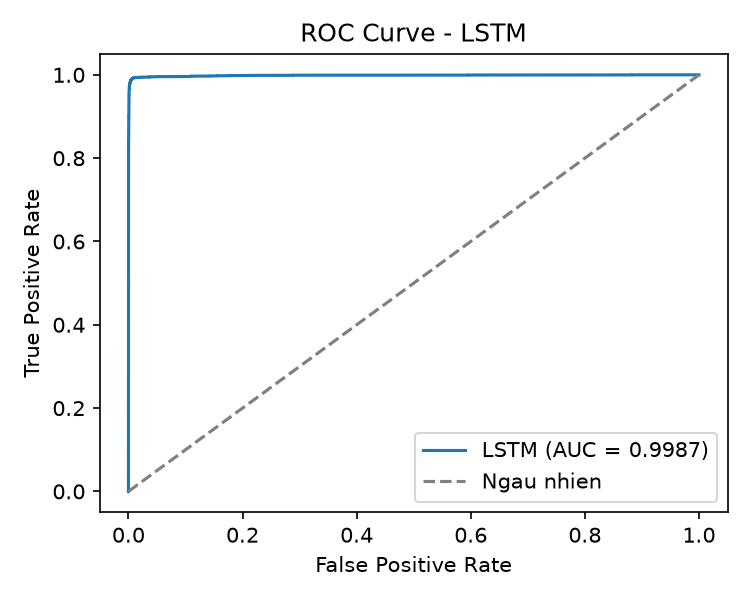
\includegraphics[width=0.75\textwidth]{images/roc-curve.png}
    \caption{Đường cong ROC của mô hình KNN trên tập kiểm tra (AUC = 0,9601)}
    \label{fig:roc}
    \Nguon{Nhóm tự thực hiện (matplotlib trên tập kiểm tra)}
\end{figure}

Đường cong ROC đi sát góc trên bên trái của đồ thị và AUC gần 0,96 cho thấy khả năng \textit{xếp hạng} của mô hình tốt hơn nhiều so với độ chính xác tại ngưỡng 0,5 mặc định: với cùng xác suất bỏ phiếu, chỉ cần \textbf{chọn ngưỡng thấp hơn} (ví dụ 0,4) hệ thống sẽ bắt được nhiều tin giả hơn, đánh đổi bằng việc gắn cờ nhầm nhiều tin thật hơn. Đây là lợi thế của cơ chế bỏ phiếu có trọng số, cho phép ``vặn'' mức nhạy cảm của hệ thống theo nhu cầu sử dụng.

\subsection{Chi phí huấn luyện và dự đoán}

Bảng \ref{tab:chi-phi} ghi lại thời gian thực đo được của từng mô hình --- chỉ số đặc biệt ý nghĩa khi so sánh KNN với các mô hình học nhiệt tình.

\begin{table}[H]
\centering
\caption{Thời gian huấn luyện và dự đoán thực đo của các mô hình}
\label{tab:chi-phi}
\begin{tabular}{|l|c|c|}
\hline
\textbf{Mô hình} & \textbf{Huấn luyện (s)} & \textbf{Dự đoán 9.777 bài (s)} \\
\hline
Naive Bayes & 0,11 & 0,02 \\
\hline
Logistic Regression & 0,42 & 0,02 \\
\hline
Passive Aggressive & 0,20 & 0,02 \\
\hline
KNN & \textbf{0,03} & 183,29 \\
\hline
\end{tabular}
\Nguon{Nhóm tự thực hiện (đo trên CPU cá nhân)}
\end{table}

Bảng này phản ánh đúng bản chất \textbf{lazy learning}: KNN ``huấn luyện'' nhanh nhất bảng (0,03 giây --- chỉ là ghi nhớ dữ liệu) nhưng dự đoán chậm nhất bảng một cách cách biệt (183,29 giây cho 9.777 bài, tương đương $\approx$ 19 ms mỗi bài), chậm hơn khoảng \textbf{9.000 lần} các mô hình tuyến tính (0,02 giây). Chi phí không biến mất mà chỉ được \textit{chuyển} từ lúc học sang mỗi lần sử dụng: mô hình tuyến tính trả ``tiền học'' một lần trong huấn luyện, KNN trả ``tiền tra cứu'' ở mọi truy vấn. Với ứng dụng demo kiểm tra từng bài riêng lẻ, 19 ms mỗi bài là chấp nhận được; nhưng ở quy mô hệ thống sàng lọc hàng triệu bài, chi phí này đòi hỏi các cấu trúc chỉ mục láng giềng gần nhất chuyên dụng (hướng phát triển ở kết luận).

\subsection{Kết quả các kịch bản thí nghiệm}

\subsubsection{E3 --- Ảnh hưởng của số láng giềng k}

Bảng \ref{tab:ket-qua-kich-ban} và hình \ref{fig:do-chinh-xac-theo-k} tổng hợp kết quả các kịch bản E3--E5.

\begin{table}[H]
\centering
\caption{Kết quả các kịch bản thí nghiệm với mô hình KNN}
\label{tab:ket-qua-kich-ban}
\begin{tabular}{|c|p{7.5cm}|c|}
\hline
\textbf{Kịch bản} & \textbf{Cấu hình} & \textbf{Accuracy (\%)} \\
\hline
E2 & Cấu hình chuẩn: $k = 5$, cosine, distance & 89,35 \\
\hline
E3 & $k = 1$ (cosine, distance) & 87,48 \\
\hline
E3 & $k = 3$ (cosine, distance) & 88,81 \\
\hline
E3 & $k = 7$ (cosine, distance) & 89,40 \\
\hline
E3 & $k = 9$ (cosine, distance) & \textbf{89,76} \\
\hline
E3 & $k = 11$ (cosine, distance) & 89,63 \\
\hline
E4 & Euclidean thay cosine ($k = 5$, distance) & 55,61 \\
\hline
E5 & Uniform thay distance ($k = 5$, cosine) & 89,25 \\
\hline
\end{tabular}
\Nguon{Nhóm tự thực hiện (cùng cách chia dữ liệu, seed cố định)}
\end{table}

\begin{figure}[H]
    \centering
    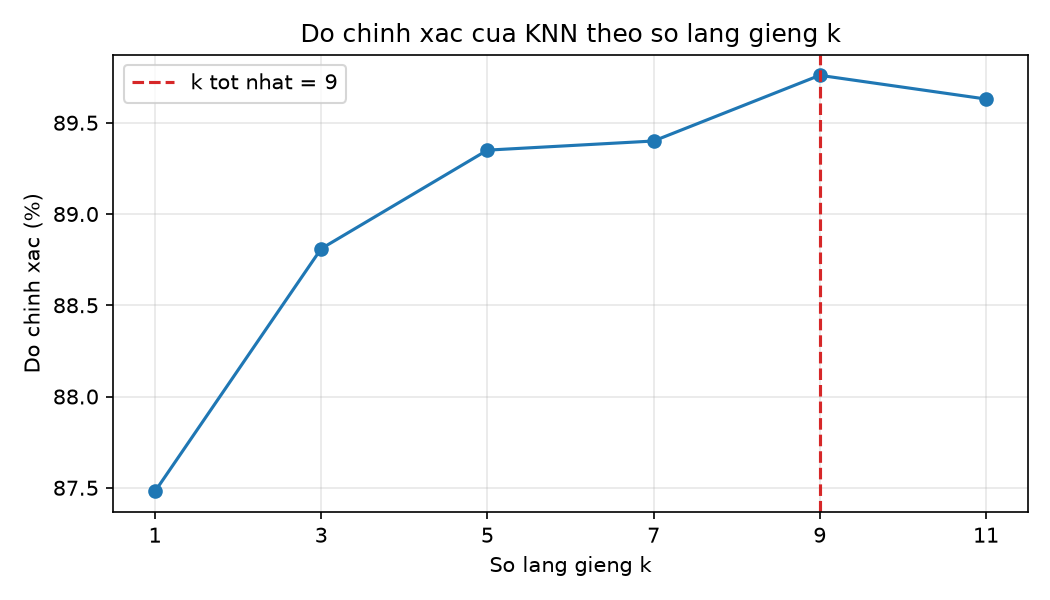
\includegraphics[width=0.85\textwidth]{images/do-chinh-xac-theo-k.png}
    \caption{Độ chính xác của KNN theo số láng giềng $k$ (kịch bản E3)}
    \label{fig:do-chinh-xac-theo-k}
    \Nguon{Nhóm tự thực hiện (matplotlib, kịch bản E3)}
\end{figure}

Từ kết quả E3 có thể rút ra:

\begin{itemize}
    \item \textbf{$k = 1$ cho kết quả thấp nhất (87,48\%)}: với một láng giềng duy nhất, dự đoán phụ thuộc hoàn toàn vào bài viết ``giống nhất'', rất nhạy với nhiễu --- một bài tin thật văn phong giật gân đủ để kéo cả dự đoán sang lớp giả. Điều này minh họa trực quan hành vi \textit{phương sai cao} phân tích ở chương 2.
    \item \textbf{Tăng $k$ làm kết quả ổn dần và đạt đỉnh tại $k = 9$ (89,76\%)}, sau đó giảm nhẹ ở $k = 11$ (89,63\%). Vùng $k = 5$--$9$ cho kết quả gần nhau (89,35\%--89,76\%), chênh lệch lớn nhất chỉ 0,41 điểm phần trăm --- nằm trong biến động ngẫu nhiên.
    \item Đề tài giữ cấu hình chuẩn \textbf{$k = 5$}: là giá trị cân bằng phổ biến trong tài liệu, nằm trong vùng ổn định, và tránh bám đuổi một đỉnh nhỏ có thể là nhiễu của tập kiểm tra cụ thể này.
\end{itemize}

\subsubsection{E4 --- Ảnh hưởng của phép đo khoảng cách}

Đây là kịch bản cho kết quả bất ngờ nhất: thay cosine bằng euclidean (cùng $k = 5$, cùng trọng số distance) làm độ chính xác \textbf{rơi từ 89,35\% xuống 55,61\%} --- gần với mức đoán theo lớp đa số (54,2\% bài tin thật). Vì theo đẳng thức \eqref{eq:l2-cos}, trên các vector chuẩn hóa L2 hai phép đo lẽ ra cho cùng thứ tự láng giềng, nhóm tiến hành chẩn đoán chi tiết và phát hiện nguyên nhân:

\begin{itemize}
    \item \textbf{Nguồn gốc vector 0}: sau tiền xử lý, một số rất ít bài viết (3 bài trong 29.328 bài huấn luyện) trở thành \textit{rỗng} (chỉ gồm từ dừng, dấu câu, chữ số\ldots) và có vector TF-IDF bằng 0 thay vì chuẩn hóa L2.
    \item \textbf{Euclidean ``mê'' vector 0}: khoảng cách euclidean từ một bài cần kiểm tra (vector chuẩn hóa, $\lVert q \rVert = 1$) tới vector 0 là $1{,}0$, trong khi khoảng cách tới các bài viết thường nằm quanh $1{,}38$--$1{,}41$ (các vector văn bản dị biệt gần như trực giao). Vì vậy các bài rỗng --- mang nhãn \textit{ngẫu nhiên} do nội dung đã bị xóa sạch --- lọt vào top-5 láng giềng của hầu hết bài kiểm tra (kiểm chứng thực đo: top-5 của euclidean chứa các láng giềng ở đúng $d = 1{,}000000$) và bỏ phiếu nhiễu vào kết quả.
    \item \textbf{Cosine miễn nhiễm}: khoảng cách cosine của vector 0 được quy ước bằng $1{,}0$ (tối đa), trong khi \textit{mọi} bài viết thật chia sẻ ít nhất một từ với bài cần kiểm tra đều có khoảng cách $< 1{,}0$ --- tức các bài rỗng luôn xếp sau toàn bộ bài có chung từ vựng và hầu như không bao giờ vào top-5.
\end{itemize}

Khi loại bỏ các bài rỗng khỏi tập huấn luyện, kết quả euclidean trở về ngang với cosine (thí nghiệm chẩn đoán trên 300 bài: trước lọc euclidean 56,33\% so với cosine 89,33\%; sau lọc euclidean 89,00\% so với cosine 89,33\% --- chênh lệch chỉ còn 0,33 điểm phần trăm), khẳng định chênh lệch 55,61\% xuất phát từ tương tác giữa \textbf{chất lượng dữ liệu} (bài rỗng) và \textbf{phép đo khoảng cách} chứ không phải từ bản chất euclidean. Bài học thực nghiệm rút ra hai lớp: (i) với văn bản, \textbf{cosine là lựa chọn bền vững} vì đo góc giữa hai vector, không bị chi phối bởi độ lớn vector; (ii) KNN đặc biệt nhạy với các mẫu nhiễu/đặc biệt trong dữ liệu --- những mẫu này không làm méo ``trọng số toàn cục'' như với mô hình tuyến tính mà trực tiếp cạnh tranh vị trí láng giềng.

\subsubsection{E5 --- Ảnh hưởng của cơ chế bỏ phiếu}

Thay bỏ phiếu đa số thuần túy (uniform) bằng bỏ phiếu có trọng số theo khoảng cách (distance) làm độ chính xác tăng nhẹ từ 89,25\% lên 89,35\%. Chênh lệch nhỏ cho thấy trong bộ dữ liệu này hai cơ chế bỏ phiếu gần tương đương; tuy nhiên trọng số theo khoảng cách vẫn được giữ làm cấu hình chuẩn vì hai lý do: (i) cho phép một láng giềng ở rất gần (bài viết gần như trùng lặp) lấn át các láng giềng ở xa, hợp lý với bản chất ``độ tương đồng''; (ii) cho ra \textbf{xác suất dự đoán mềm} liên tục --- điều kiện cần để vẽ đường cong ROC và linh hoạt điều chỉnh ngưỡng cảnh báo như đã phân tích.

\subsubsection{E6 --- So sánh Bag-of-Words và TF-IDF}

Đề cương yêu cầu thử nghiệm cả hai cách biểu diễn văn bản cơ bản. Nhóm giữ nguyên dữ liệu, phép tiền xử lý và cách chia tập, chỉ đổi vector hóa: \textbf{Bag-of-Words} (CountVectorizer --- đếm số lần từ xuất hiện) và \textbf{TF-IDF} (TfidfVectorizer --- nhân thêm trọng số nghịch tần suất tài liệu, mục \ref{sec:tfidf}). Mỗi cách được thử với unigram và 1--2gram, thay đổi min\_df và số đặc trưng tối đa; với mỗi cấu hình, nhóm huấn luyện MultinomialNB (mốc so sánh) và KNN ($k = 5$, cosine, distance). Kết quả ở bảng \ref{tab:bieu-dien} và hình \ref{fig:so-sanh-bieu-dien}.

\begin{table}[H]
\centering
\caption{So sánh Bag-of-Words và TF-IDF trên cùng một cách chia dữ liệu (tập kiểm tra 9.777 bài)}
\label{tab:bieu-dien}
\small
\begin{tabular}{|l|l|l|r|r|r|r|}
\hline
\textbf{Biểu diễn} & \textbf{Cấu hình} & \textbf{Mô hình} & \textbf{Acc (\%)} & \textbf{F1 (\%)} & \textbf{Số chiều} & \textbf{Dự đoán (s)} \\
\hline
BoW & BoW unigram & NB & 95,97 & 95,47 & 154.464 & 0,0 \\ \hline
BoW & BoW 1-2gram & NB & \textbf{96,68} & \textbf{96,23} & 2.846.173 & 0,4 \\ \hline
TF-IDF & TF-IDF unigram & NB & 93,38 & 92,28 & 154.464 & 0,0 \\ \hline
TF-IDF & TF-IDF 1-2gram & NB & 95,81 & 95,35 & 50.000 & 0,0 \\ \hline
TF-IDF & TF-IDF min_df=3 & NB & 95,82 & 95,36 & 50.000 & 0,0 \\ \hline
TF-IDF & TF-IDF 20.000 đặc trưng & NB & 95,63 & 95,16 & 20.000 & 0,0 \\ \hline
BoW & BoW 1-2gram & KNN & 87,94 & 84,82 & 2.846.173 & 77,8 \\ \hline
TF-IDF & TF-IDF 1-2gram & KNN & \textbf{89,35} & \textbf{87,45} & 50.000 & 43,9 \\ \hline
\end{tabular}
\Nguon{Nhóm tự thực hiện (results/bieu-dien.json, random_state = 42)}
\end{table}

\begin{figure}[H]
    \centering
    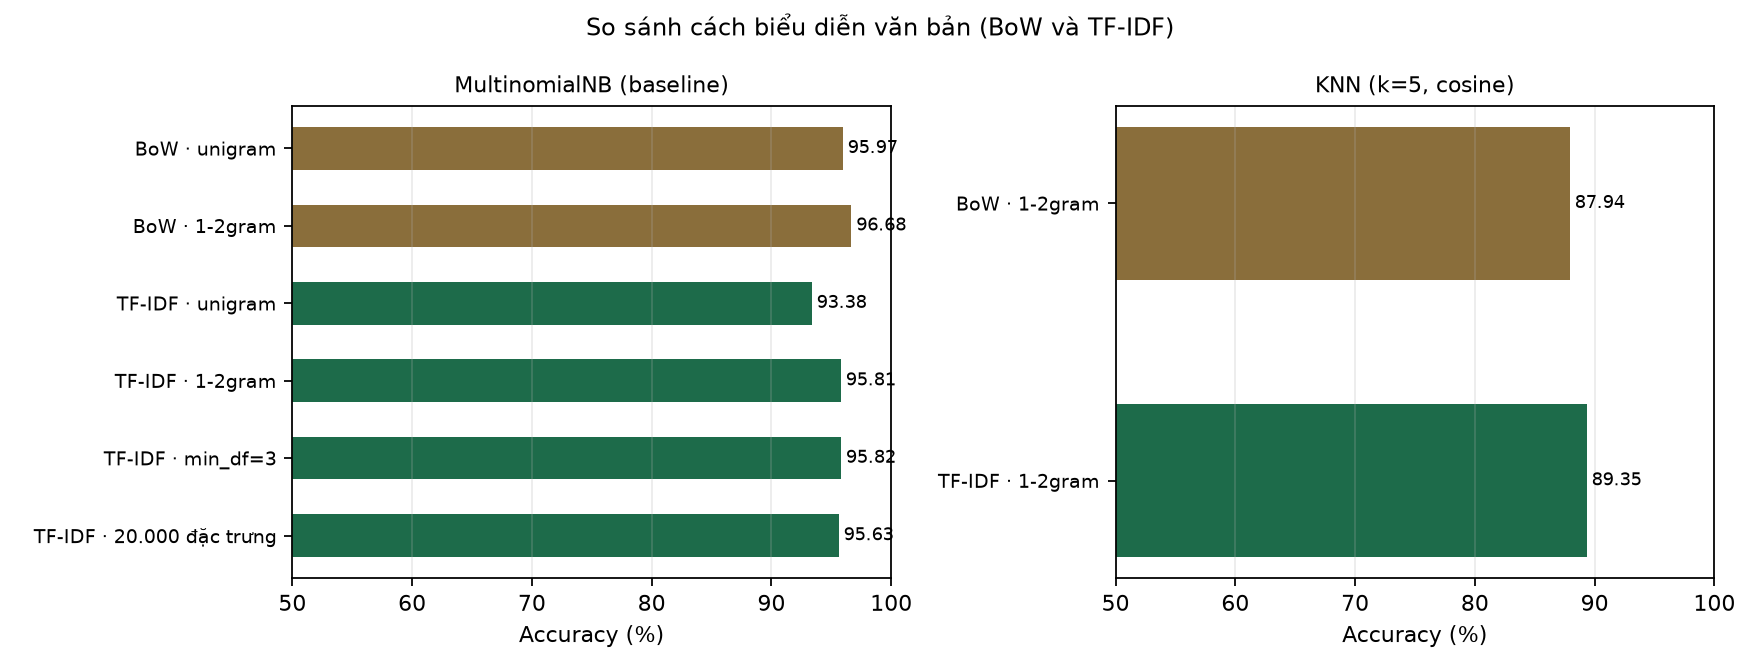
\includegraphics[width=0.9\textwidth]{images/so-sanh-bieu-dien.png}
    \caption{Độ chính xác theo cách biểu diễn văn bản, cho MultinomialNB và KNN}
    \label{fig:so-sanh-bieu-dien}
    \Nguon{Nhóm tự thực hiện (matplotlib, kịch bản experiments\_representation.py)}
\end{figure}

Từ bảng \ref{tab:bieu-dien} rút ra bốn nhận xét:

\begin{itemize}
    \item \textbf{1--2gram luôn tốt hơn unigram.} Với NB, TF-IDF tăng từ 93,38\% lên 95,81\% khi thêm bigram; với BoW, từ 95,97\% lên 96,68\%. Cặp từ giữ lại được những cụm có sức phân loại như tên tổ chức, hãng tin hay ``fake news''.
    \item \textbf{BoW thắng TF-IDF ở mô hình tuyến tính.} BoW 1--2gram đạt 96,68\%, cao hơn TF-IDF 1--2gram (95,81\%) dù dùng tới 2.846.173 chiều so với 50.000. Trong bộ ISOT, sự lặp lại của tên hãng tin và cú pháp giật gân chính là tín hiệu phân loại; TF-IDF hạ trọng số từ xuất hiện thường xuyên nên làm mất một phần tín hiệu này. Kết quả này cho thấy TF-IDF không phải lúc nào cũng vượt BoW --- cần thử nghiệm trên chính tập dữ liệu của đề tài.
    \item \textbf{min\_df và số đặc trưng có tác động nhỏ.} Đặt min\_df = 3 cho accuracy 95,82\%, gần như không đổi so với 95,81\%, vì max\_features = 50.000 đã loại bỏ phần lớn n-gram hiếm từ trước. Giảm xuống 20.000 chiều làm accuracy giảm nhẹ xuống 95,63\%, đổi lại ma trận gọn hơn.
    \item \textbf{Với KNN, ưu tiên TF-IDF.} Cấu hình KNN tốt nhất trong bảng là TF-IDF 1-2gram với accuracy 89,35\%. Dự đoán của KNN phải tính khoảng cách tới 29.328 bài huấn luyện, nên chi phí tăng nhanh theo số chiều; TF-IDF 50.000 chiều giữ độ chính xác gần BoW nhưng bộ nhớ và thời gian dự đoán thấp hơn đáng kể. Đây là lý do nhóm chọn TF-IDF cho mô hình chính và cho giao diện demo.
\end{itemize}

\subsection{Phân tích lỗi phân loại}

Mô hình KNN phân loại sai 1.041 bài trên 9.777 bài kiểm tra, trong đó \textbf{778 bài tin giả bị nhận nhầm thành tin thật} (chiếm 75\% tổng số lỗi) và 263 bài tin thật bị nhầm thành giả. Nhóm tổng hợp các nhóm lỗi phổ biến quan sát được trong quá trình thử nghiệm (bảng \ref{tab:phan-tich-loi}).

\begin{table}[H]
\centering
\caption{Tóm tắt các nhóm lỗi phân loại phổ biến}
\label{tab:phan-tich-loi}
\begin{tabular}{|p{4.5cm}|p{5cm}|p{3.5cm}|}
\hline
\textbf{Nhóm lỗi} & \textbf{Đặc điểm} & \textbf{Nguyên nhân có thể} \\
\hline
Tin giả văn phong gần báo chí chính thống & Viết theo cấu trúc bài chuẩn, dùng từ vựng chủ đề chính trị trùng với tin thật & Láng giềng gần nhất đa số là tin thật; KNN quyết theo số đông cục bộ \\
\hline
Bài ngắn, ít thông tin & Tiêu đề ngắn, nội dung 1--2 câu & Vector thưa, ít tín hiệu tương đồng để xác định láng giềng đáng tin \\
\hline
Tin thật văn phong giật gân & Tiêu đề câu chú ý, từ ngữ cảm thán & Bị ``kéo'' về phía các bài tin giả văn phong tương tự \\
\hline
Bài rỗng sau tiền xử lý & Nội dung chỉ gồm từ dừng, dấu câu, chữ số & Vector 0; láng giềng gần như ngẫu nhiên (phân tích E4) \\
\hline
\end{tabular}
\Nguon{Nhóm tự phân tích trên tập kiểm tra}
\end{table}

Nhận xét trên cho thấy mô hình chủ yếu phân biệt hai lớp qua \textbf{độ tương đồng từ vựng} hơn là kiểm chứng sự thật của nội dung. Đây là giới hạn cố hữu của phương pháp phân loại văn bản thuần túy, đồng thời gợi ý hướng cải tiến: làm sạch kỹ hơn dữ liệu (loại bài rỗng), kết hợp thông tin nguồn tin hoặc kiểm chứng chéo đa bài viết.

\section{Nhận xét và thảo luận}
\label{sec:nhan-xet}

\textbf{Ưu điểm của KNN trong đề tài:}

\begin{itemize}
    \item \textbf{Đơn giản và không cần huấn luyện}: toàn bộ ``tri thức'' của mô hình là chính bộ dữ liệu đã gán nhãn; thêm bài tin mới được xác thực chỉ là thêm một mẫu lưu trữ, không cần huấn luyện lại.
    \item \textbf{Dễ diễn giải} --- lợi thế nổi bật cho bài toán phát hiện tin giả: với mỗi dự đoán, hệ thống có thể chỉ ra ngay \textbf{5 bài viết gần nhất} và nhãn của chúng làm căn cứ, giúp người kiểm duyệt kiểm tra lại quyết định của máy. Các mô hình tuyến tính chỉ cho biết ``trọng số từ nào đẩy dự đoán'', khó trực quan hơn nhiều.
    \item \textbf{Ngưỡng quyết định linh hoạt}: cơ chế bỏ phiếu có trọng số cho xác suất mềm, AUC 0,9601 cho phép điều chỉnh độ nhạy của hệ thống theo nhu cầu (bắt chặt hơn hoặc ít báo động giả hơn).
    \item Trên bộ dữ liệu thí nghiệm, KNN đạt 89,35\% \textit{mà không cần học gì cả} --- mọi hiệu năng đến từ so khớp trực tiếp, cho thấy độ phân tách tự nhiên của hai lớp theo từ vựng.
\end{itemize}

\textbf{Nhược điểm và chi phí:}

\begin{itemize}
    \item \textbf{Độ chính xác thấp nhất bảng} (89,35\%, thấp hơn Passive Aggressive 10,02 điểm phần trăm), đặc biệt recall trên lớp tin giả chỉ 82,34\% --- khoảng 1/5 tin giả bị bỏ sót, loại sai nguy hiểm nhất của hệ thống phát hiện tin giả.
    \item \textbf{Dự đoán rất chậm}: 183,29 giây cho 9.777 bài so với 0,02 giây của mô hình tuyến tính (gấp $\approx$ 9.000 lần) do đặc tính lazy learning --- mỗi truy vấn phải quét toàn bộ 29.328 bài huấn luyện. Bộ nhớ lưu mô hình cũng lớn hơn nhiều vì phải giữ nguyên toàn bộ ma trận đặc trưng tập huấn luyện.
    \item \textbf{Nhạy cảm với dữ liệu nhiễu và lựa chọn siêu tham số}: thí nghiệm E4 cho thấy chỉ 3 bài rỗng (0,01\% dữ liệu) cộng với phép đo euclidean đã khiến độ chính xác rơi xuống 55,61\%; E3 cho thấy $k$ nhỏ làm kết quả giảm rõ (87,48\% tại $k = 1$).
\end{itemize}

\textbf{Vì sao các mô hình tuyến tính TF-IDF vượt trội trên bộ dữ liệu này?} Với đặc trưng TF-IDF, các từ mang dấu hiệu nguồn (tên chủ đề, văn phong tin chính thống Reuters, kiểu tiêu đề giật gân\ldots) có trọng số rất cao; Logistic Regression và Passive Aggressive học một \textbf{ranh giới toàn cục} trong không gian đặc trưng, tận dụng trực tiếp tín hiệu đó và phân tách hai lớp gần như hoàn hảo (99,37\%). KNN không học ranh giới mà so khớp cục bộ: một bài tin giả viết gần văn phong báo chí chính thống sẽ có láng giềng đa số là tin thật và bị bỏ sót. Kết quả này một mặt xác nhận bộ dữ liệu ISOT ``dễ'' với mô hình dựa trên tần suất từ (hiện tượng ``rò rỉ nguồn tin''), mặt khác cho thấy điểm yếu đặc hữu của KNN trên dữ liệu thưa chiều cao --- đúng như phân tích lý thuyết ở chương 2 về lời nguyền chiều và tầm quan trọng của phép đo khoảng cách.

\textbf{So sánh với các nghiên cứu khác trên cùng bộ dữ liệu:} nghiên cứu gốc \cite{ahmed2017} đạt khoảng 93\% với Passive Aggressive; các nghiên cứu công bố trên ISOT với mô hình học sâu (LSTM, CNN) thường đạt 98--99\% và trên 99\% với BERT \cite{bert}. Kết quả ba mô hình tham chiếu của nhóm (95,81\%--99,37\%) nằm trong vùng này và cao hơn nghiên cứu gốc, chủ yếu do khác biệt tiền xử lý (loại từ dừng, Porter Stemmer, loại bỏ bài trùng lặp) và cách chia tập huấn luyện/kiểm tra. KNN 89,35\% ở dưới vùng đó --- đúng như bản chất của thuật toán trên đặc trưng túi từ, và là căn cứ cho các hướng cải tiến ở kết luận (giảm chiều, biểu diễn ngữ nghĩa, chỉ mục láng giềng nhanh).

\section{Ứng dụng thử nghiệm}

Để minh họa khả năng ứng dụng thực tế, nhóm xây dựng một giao diện demo nhỏ bằng thư viện \textbf{Streamlit} (Python): người dùng dán nội dung một bài tin tức bất kỳ vào khung văn bản, hệ thống nạp mô hình KNN đã xây dựng (kèm vectorizer TF-IDF), tiền xử lý đúng như lúc xây dựng mô hình và hiển thị dự đoán kèm xác suất (Hình \ref{fig:demo-streamlit-1} và Hình \ref{fig:demo-streamlit-2}).

{\small
\begin{verbatim}
# app.py --- Demo phat hien tin gia bang Streamlit (KNN)
import pickle
import streamlit as st

with open("knn_model.pkl", "rb") as f:
    model = pickle.load(f)
with open("tfidf_vectorizer.pkl", "rb") as f:
    vectorizer = pickle.load(f)

st.title("Kiem tra tin that hay tin gia")
text = st.text_area("Dan noi dung bai viet vao day:")

if st.button("Kiem tra"):
    x = vectorizer.transform([clean_text(text)])
    p = float(model.predict_proba(x)[0][1])
    if p >= 0.5:
        st.error(f"CANH BAO: kha nang tin GIA la {p:.1%}")
    else:
        st.success(f"Ket qua: kha nang tin THAT la {1-p:.1%}")
\end{verbatim}
}

\begin{figure}[H]
    \centering
    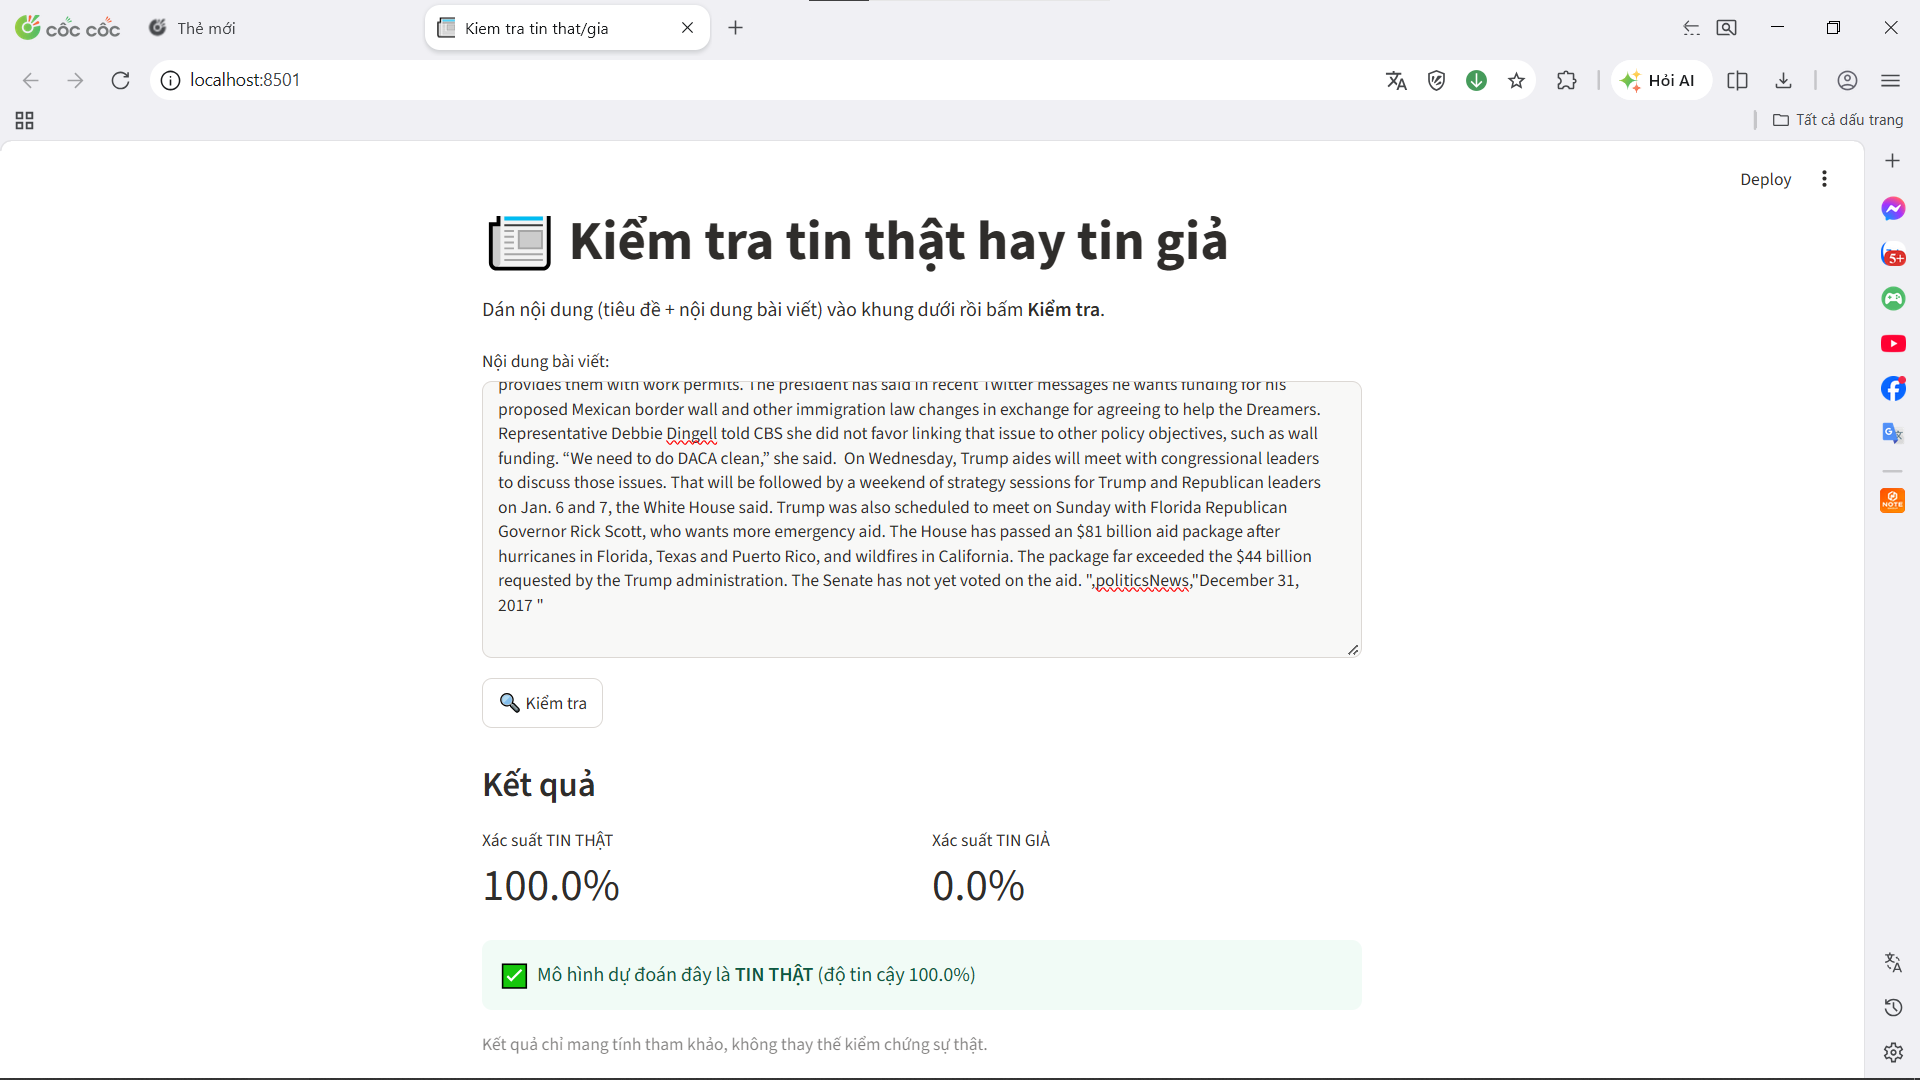
\includegraphics[width=\textwidth]{images/demo-streamlit-1.png}
    \caption{Giao diện demo kiểm tra một bài tin thật: mô hình dự đoán đúng là tin thật với độ tin cậy 100\%}
    \label{fig:demo-streamlit-1}
    \Nguon{Nhóm tự thực hiện}
\end{figure}

\begin{figure}[H]
    \centering
    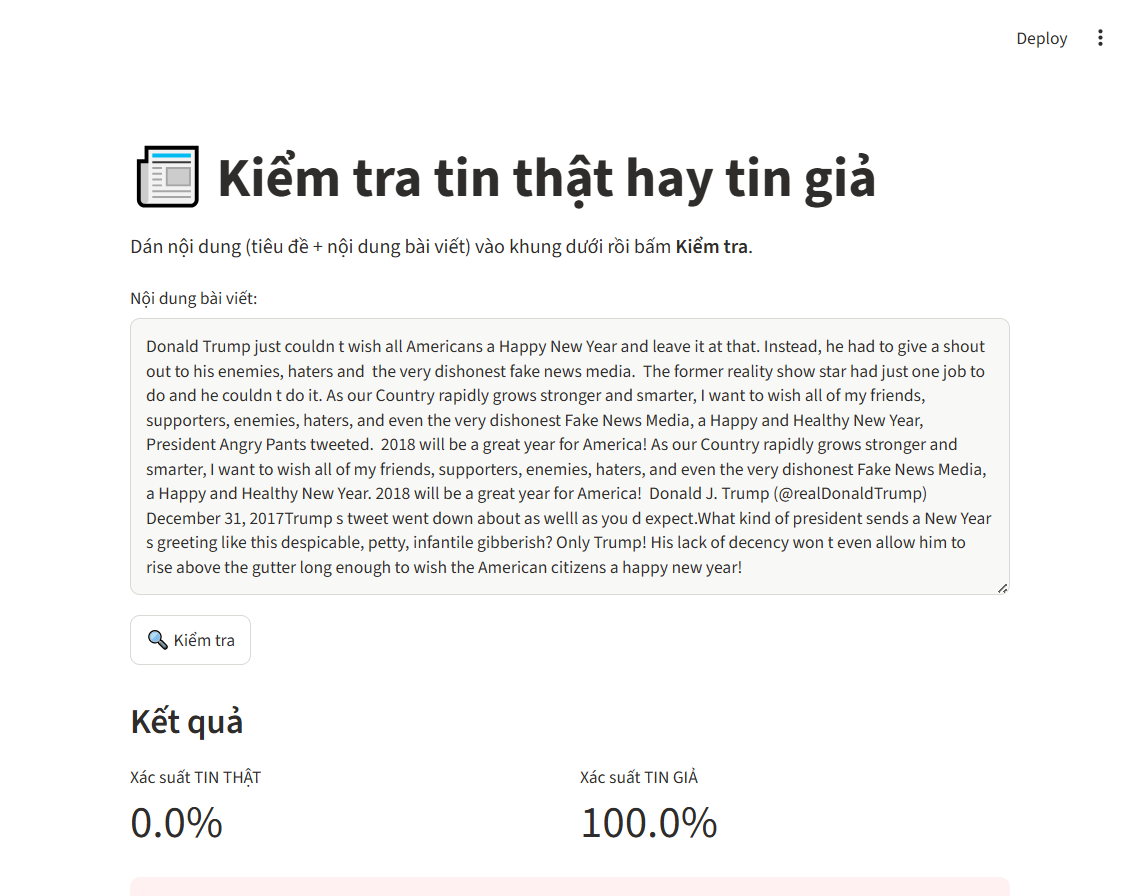
\includegraphics[width=\textwidth]{images/demo-streamlit-2.png}
    \caption{Giao diện demo kiểm tra một bài tin giả: mô hình cảnh báo đúng là tin giả với độ tin cậy 100\%}
    \label{fig:demo-streamlit-2}
    \Nguon{Nhóm tự thực hiện}
\end{figure}

Trong cả hai trường hợp thử nghiệm (một bài tin thật và một bài tin giả lấy từ bộ dữ liệu ISOT), mô hình dự đoán đúng với độ tin cậy 100\%. Ứng dụng demo tuy đơn giản nhưng cho thấy mô hình có thể được tích hợp vào các hệ thống thực tế: tiện ích trình duyệt hỗ trợ người đọc, hệ thống lọc nội dung cho mạng xã hội, hoặc công cụ hỗ trợ biên tập viên báo chí kiểm tra nguồn tin trước khi trích dẫn; chi phí dự đoán $\approx$ 19 ms mỗi bài (bảng \ref{tab:chi-phi}) đủ nhanh cho tương tác đơn bài.
